\documentclass[spanish, letterpaper,12]{article}\usepackage[]{graphicx}\usepackage[]{xcolor}
% maxwidth is the original width if it is less than linewidth
% otherwise use linewidth (to make sure the graphics do not exceed the margin)
\makeatletter
\def\maxwidth{ %
  \ifdim\Gin@nat@width>\linewidth
    \linewidth
  \else
    \Gin@nat@width
  \fi
}
\makeatother

\definecolor{fgcolor}{rgb}{0.345, 0.345, 0.345}
\newcommand{\hlnum}[1]{\textcolor[rgb]{0.686,0.059,0.569}{#1}}%
\newcommand{\hlsng}[1]{\textcolor[rgb]{0.192,0.494,0.8}{#1}}%
\newcommand{\hlcom}[1]{\textcolor[rgb]{0.678,0.584,0.686}{\textit{#1}}}%
\newcommand{\hlopt}[1]{\textcolor[rgb]{0,0,0}{#1}}%
\newcommand{\hldef}[1]{\textcolor[rgb]{0.345,0.345,0.345}{#1}}%
\newcommand{\hlkwa}[1]{\textcolor[rgb]{0.161,0.373,0.58}{\textbf{#1}}}%
\newcommand{\hlkwb}[1]{\textcolor[rgb]{0.69,0.353,0.396}{#1}}%
\newcommand{\hlkwc}[1]{\textcolor[rgb]{0.333,0.667,0.333}{#1}}%
\newcommand{\hlkwd}[1]{\textcolor[rgb]{0.737,0.353,0.396}{\textbf{#1}}}%
\let\hlipl\hlkwb

\usepackage{framed}
\makeatletter
\newenvironment{kframe}{%
 \def\at@end@of@kframe{}%
 \ifinner\ifhmode%
  \def\at@end@of@kframe{\end{minipage}}%
  \begin{minipage}{\columnwidth}%
 \fi\fi%
 \def\FrameCommand##1{\hskip\@totalleftmargin \hskip-\fboxsep
 \colorbox{shadecolor}{##1}\hskip-\fboxsep
     % There is no \\@totalrightmargin, so:
     \hskip-\linewidth \hskip-\@totalleftmargin \hskip\columnwidth}%
 \MakeFramed {\advance\hsize-\width
   \@totalleftmargin\z@ \linewidth\hsize
   \@setminipage}}%
 {\par\unskip\endMakeFramed%
 \at@end@of@kframe}
\makeatother

\definecolor{shadecolor}{rgb}{.97, .97, .97}
\definecolor{messagecolor}{rgb}{0, 0, 0}
\definecolor{warningcolor}{rgb}{1, 0, 1}
\definecolor{errorcolor}{rgb}{1, 0, 0}
\newenvironment{knitrout}{}{} % an empty environment to be redefined in TeX

\usepackage{alltt}

\usepackage{amsmath}
\usepackage{amssymb}
\usepackage{graphicx}
\usepackage{verbatim}
\usepackage{hyperref}
\usepackage{eurosym}
\usepackage[numbers]{natbib}
\usepackage{enumitem}

\usepackage[activeacute]{babel}
\usepackage[utf8x]{inputenc}
\usepackage[T1]{fontenc}
\spanishdecimal{.}

\DeclareGraphicsExtensions{.pdf, .png}
\graphicspath{{./fig/}}

\title{Curso Básico de R}
\author{Dr. Isaías Moreno Cruz}
\date{\today}

%----------------------------------------------------------------------
\IfFileExists{upquote.sty}{\usepackage{upquote}}{}
\begin{document}                                                      
\SweaveOpts{concordance=TRUE}
%----------------------------------------------------------------------
\renewcommand{\tablename}{Tabla}

\maketitle

\section{Install R packages}


knitr
xtable


\section{Introducción}
\label{sec:intro}


\subsection{Operaciones vectorizadas}
\label{subsec:operaciones_vectorizadas}

Muchas operaciones en R son vectorizadas, haciendo el código más eficiente, conciso, y fácil de leer.

\begin{knitrout}
\definecolor{shadecolor}{rgb}{0.969, 0.969, 0.969}\color{fgcolor}\begin{kframe}
\begin{alltt}
\hldef{x} \hlkwb{<-} \hlnum{1}\hlopt{:}\hlnum{4}\hldef{; y} \hlkwb{<-} \hlnum{6}\hlopt{:}\hlnum{9}
\hldef{x}\hlopt{+}\hldef{y}
\end{alltt}
\begin{verbatim}
## [1]  7  9 11 13
\end{verbatim}
\end{kframe}
\end{knitrout}


\begin{knitrout}
\definecolor{shadecolor}{rgb}{0.969, 0.969, 0.969}\color{fgcolor}\begin{kframe}
\begin{alltt}
\hldef{x} \hlopt{>} \hlnum{2}
\end{alltt}
\begin{verbatim}
## [1] FALSE FALSE  TRUE  TRUE
\end{verbatim}
\end{kframe}
\end{knitrout}

\begin{knitrout}
\definecolor{shadecolor}{rgb}{0.969, 0.969, 0.969}\color{fgcolor}\begin{kframe}
\begin{alltt}
\hldef{x}\hlopt{/}\hldef{y}
\end{alltt}
\begin{verbatim}
## [1] 0.1666667 0.2857143 0.3750000 0.4444444
\end{verbatim}
\end{kframe}
\end{knitrout}

El valor de y[1]=6.



\subsection{Operaciones con matrices}

\begin{knitrout}
\definecolor{shadecolor}{rgb}{0.969, 0.969, 0.969}\color{fgcolor}\begin{kframe}
\begin{alltt}
\hldef{x} \hlkwb{<-} \hlkwd{matrix}\hldef{(}\hlnum{1}\hlopt{:}\hlnum{4}\hldef{,}\hlnum{2}\hldef{,}\hlnum{2}\hldef{); y} \hlkwb{<-} \hlkwd{matrix}\hldef{(}\hlkwd{rep}\hldef{(}\hlnum{10}\hldef{,}\hlnum{4}\hldef{),}\hlnum{2}\hldef{,}\hlnum{2}\hldef{)}
\hldef{x} \hlopt \hldef{y} \hlcom{# multiplicaciones de matrices}
\end{alltt}
\begin{verbatim}
##      [,1] [,2]
## [1,]   40   40
## [2,]   60   60
\end{verbatim}
\end{kframe}
\end{knitrout}



\section{Leer y escribir datos}
\label{sec:datos}


\subsection{Leer una gran base de datos con read.table}

Con una base de datos grande, hacer lo siguiente te hará la vida más fácil y previene que R detenga.
\begin{itemize}
 \item Lee la pagina de ayuda de \verb=read.table=, la cual contiene muchos consejos.
 \item Haz un calculo aproximado de la memoria que requiere almacenar tu base de datos. Si el conjunto de datos es más grande que la cantidad de memoria RAM en tu computadora , probablemente debes detenerte.
 \item Utiliza \verb=comment.char=" si no hay lineas de comentarios en el archivo.
 \item Usa el argumento \verb=colClasses=. Especifica esta opción en lugar de usar la de pordefecto puede hacer \verb=read.table= mucho más rápido, frecuentemente hasta dos veces más rapido. Si todas las columnas son \verb=numeric=, entonces puedes usar \verb$colClasses="numeric"$.
 \item \verb=nrows=. Esta no hace a R más rápida pero ayuda con el uso de la memoria. Puedes usar el comando de Unix \verb=wc= para calcular el numero de lineas en el archivo. 
\end{itemize}


Una rápida forma, aunque poco elegante, de conocer la clase de cada columna es la siguiente:
\begin{verbatim}
initial <- read.table("data.txt", nrows=100)
classes <- sapply(initial, class)
tabAll <- read.table("data.txt", colClasses= classes)
\end{verbatim}



\begin{kframe}
\begin{alltt}
  \hlkwd{library}\hldef{(xtable)}
  \hlkwd{xtable}\hldef{(}\hlkwd{head}\hldef{(df))}
\end{alltt}
\end{kframe}% latex table generated in R 4.4.1 by xtable 1.8-4 package
% Mon Oct 14 18:02:36 2024
\begin{table}[ht]
\centering
\begin{tabular}{rrrrr}
  \hline
 & ozone & radiation & temperature & wind \\ 
  \hline
1 & 41.00 & 190.00 & 67.00 & 7.40 \\ 
  2 & 36.00 & 118.00 & 72.00 & 8.00 \\ 
  3 & 12.00 & 149.00 & 74.00 & 12.60 \\ 
  4 & 18.00 & 313.00 & 62.00 & 11.50 \\ 
  5 & 23.00 & 299.00 & 65.00 & 8.60 \\ 
  6 & 19.00 & 99.00 & 59.00 & 13.80 \\ 
   \hline
\end{tabular}
\end{table}




\subsection{Figure}
\label{subsec:fig}

  
  \begin{figure}[h!]
  \centering
\begin{knitrout}
\definecolor{shadecolor}{rgb}{0.969, 0.969, 0.969}\color{fgcolor}
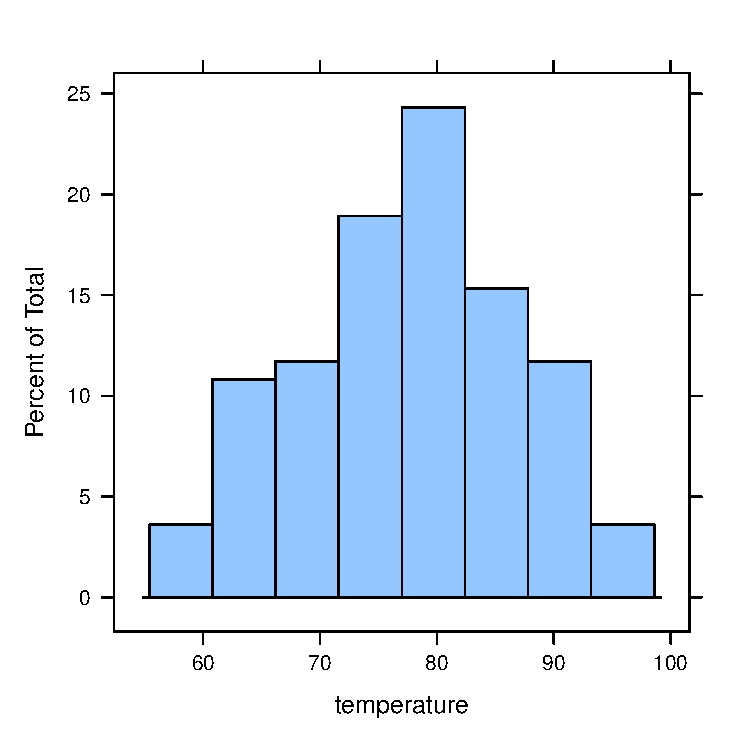
\includegraphics[width=\maxwidth]{figure/my-label-1} 
\end{knitrout}
  \caption{\label{fig:Dname} Descripción.}
\end{figure}


%----------------------------------------------------------------------
\end{document}
%----------------------------------------------------------------------
